
\chapter{The ``cells" of an OO program}
\label{ch:cells}

Java is called an ``object-oriented" programming language. If I were King of
the World, I would have called it a ``\textit{class}-oriented" language
instead. That's because in Java, you don't write code for objects, but for
\textit{classes}, and that code then defines the behavior of the classes that
are based on them.\footnote{There are other languages, for instance JavaScript
(no relation to Java), which do deserve the term ``\textit{object}-oriented,"
since you can create code for individual objects rather than classes, and not
every object has to have a class at all.} You'll sometimes hear people
mistakenly say stuff like, ``I wrote some code for the DatabaseConnection
object today." It makes me wince. They weren't writing ``code for the
object," but the code for a class.

If an OO program is an organic entity, classes and objects comprise its cells.

\section{Terms}

So here's a crucial pair of definitions. A \textbf{class} is a
\textit{category} of things. An \textbf{object} is a concrete \textit{example}
of a class. If ``University" is a class, then ``UMW" is an object; if
``Course" is a class, then ``CPSC 240" is an object. The difference is real,
and it is vitally important to keep at the forefront of your mind as you begin
your OO quest. Getting them mixed up is like Peter Venkman crossing the
streams.

You'll sometimes hear alternate definitions of these terms, like ``a class is
a template, and objects are copies of that template." This is better than
out-and-out confusion, but it still misses something important. It's an
operational definition, instead of a conceptual definition. It thinks of a
class and an object in terms of the mechanical way the virtual machine carries
out their duties, rather than in terms of \textit{modeling}, which is what
OOA\&D is all about.

In our world, every single software object will be a member of a category,
and that category will define everything about its inner structure and rules
of behavior.

By the way, an important near-synonym for class is \textbf{type}. (It's only a
\textit{near}-synonym because primitive, non-classes like \texttt{int}s and
\texttt{boolean}s are also types.) An important exact synonym for object is
\textbf{instance}.

In addition to those nouns, a big verb in our vocabulary will be the term
\textbf{instantiate}. It means ``to actually create an object of a particular
class." Some people use words like \textbf{construct} or \textbf{create} for
this, or even ``\texttt{new}" (or ``\texttt{new} up") as a verb, but for the
most part we'll stick with instantiate.


\section{A different kind of language}
\label{sec:UMLclasses}

Classes and objects are among the basic building blocks of any OO program, and
they will play a prominent role on various \textbf{UML diagrams}. UML
(``Unified Modeling Language") is a \textit{design} language, not a
programming language. It is expressed in visual diagrams, not streams of text.
Even though it's not text-based, though, and even though there's no
``compiler" forcing us to adhere to the syntax, it still has rules that must
be followed, and precise meanings that can be inferred.

Figure~\ref{fig:classObject} shows what a class, and an object, look like in
UML. (I'm putting classes in yellow and objects in blue, but those colors
aren't part of UML itself, just the black-and-white stuff.) Both are boxes,
but notice the class box has three compartments in it while the object box has
two.

\begin{figure}[ht]
\centering
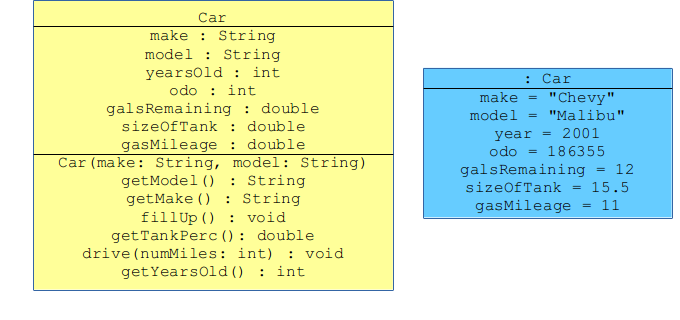
\includegraphics[width=1.0\textwidth]{classObject.pdf}   % 650x350
\caption{A class (left) and an object in UML.}
\label{fig:classObject}
\end{figure}

\subsection{Classes in UML: the first two compartments}

Let's look at the class in detail. In the top box is its name; so far so good.
One thing to point out, though, is that in Java, \textit{the names of all
classes are capitalized.} Don't ever violate this rule, for convention's and
confusion's sake!

The second compartment has the class's \textbf{instance variables}. You'll
hear people use other terms for these like like ``member variables" and even
``class variables," but I strongly prefer instance variables (or ``inst vars"
for short) and here's why: \textit{every instance has its own copy of an
instance variable.} This truth is absolutely fundamental to OOP, and it's
worth re-reading that sentence again and again until it's part of your core
being. Declaring a plain-ol' variable like ``\texttt{int x;}" creates a single
storage location in which a value can be stored. But declaring an
\textit{instance} variable is a far-reaching choice that destines every Car
(or whatever) that will come about in the future to have its own copy of that
variable. It's our way of defining the very structure of Cars in perpetuity.

One slight headache is that the UML syntax differs from Java's a bit: instead
of listing the variable's type and then its name, we reverse them, we use
a colon instead of a space, and we omit the semicolon. Otherwise, it's pretty
straightforward to interpret that second compartment.

By the way, one important piece of syntax in that second compartment is an
\underline{underline}, which says that the underlined ``instance variable"
isn't an instance variable after all: it's a \textbf{class variable}. This
means that \textit{there's only one shared variable for the entire class,
rather than a different variable for each object.} In
Figure~\ref{fig:classObject}, the integer \texttt{numCars} variable is such a
case. Even though every \texttt{Car} has its own \texttt{make},
\texttt{model}, \texttt{odo}meter reading, \textit{etc.}, they all share one
\texttt{numCars} (which presumably represents the total number of \texttt{Car}
objects instantiated so far.) This makes sense, since after all such a
variable is not specific to a certain \texttt{Car}. We'll see that in Java,
class variables are created by using the ``\texttt{static}" keyword where the
variable is declared.

\subsection{Classes in UML: the third compartment}

The third compartment isn't much harder: it contains the \textbf{methods} for
the class. Like everything it seems, programmers have multiple terms for these
two: they're called \textbf{member functions} or \textbf{class functions} on
occasion. We'll stick with \textbf{method}.

The crucial distinction between a method and a regular ol' Joe function is
this: while you can call a function to trigger it, you must call a method
\textit{on an object}. In the example, we have a \texttt{fillUp()} method
defined on the \texttt{Car} class. Since it's not an ordinary function, but
rather an OO method, we must call it on a particular instance of a
\texttt{Car}. In Java code, this does \textit{not} work:

\begin{verbatim}
    fillUp();        // NOPE
\end{verbatim}

nor does this:

\begin{verbatim}
    Car.fillUp();    // NOPE
\end{verbatim}

Instead, one must call \texttt{fillUp()} like this:

\begin{verbatim}
    johnsMercedes.fillUp();     // Correct!
\end{verbatim}

where \texttt{johnsMercedes} is the name of a valid \texttt{Car} object,
previously instantiated.

Beginners sometimes view this as a syntactic nuisance. It is not. It is
fundamental to what your code \textit{means}. Conceptually, it makes sense to
have a particular car, and to fill it up. It does \textit{not} make sense to
say ``hey universe, fill up cars" (which is what ``\texttt{fillUp()}" seems to
say) not to say ``hey Cars-in-general, fill yourself up" (which is what
``\texttt{Car.fillUp()}" seems to say).

By the way, notice in the example I just gave, \texttt{johnsMercedes} is
\textit{not} capitalized. (The capital ``\texttt{M}" in the middle doesn't
count; that's just an artifact of CamelCase, which is a way of making multiple
words easier to read.) This is always the case: in Java, object names always
begin with a lower-case letter.

Back to the third compartment. You can probably tell that the stuff inside the
parentheses is arguments to the respective methods, with the same
name-first-then-type colon-syntax, and you can probably tell that after the
closing parenthesis, you have the return type of the function. All of this
looks vaguely Java-like, and that's because even though a UML diagram is
technically programming-language-independent, language-specific things like
\texttt{int} and \texttt{String} can't help but creep in in practice. Our
thoughts betray us.

\subsubsection{Various ``special" methods}

A few of those methods are worthy of special note. The first one listed,
called simply ``\texttt{Car}", is a very special kind of method called a
\textbf{constructor} which we'll be talking about a lot. Here's an iron-clad
rule which is fundamental to much that follows: \textit{whenever an object is
instantiated, one of its class's constructors is called.} This happens
automatically; it's not something we have to do ourselves. (Java's syntax for
this, as we'll see, makes it kind of look like we're calling the constructor
ourselves, which is a mixed blessing.) In Java, there are two things that
``make" a method a constructor: (1) it must have exactly the same name as the
class, and (2) it must have \textit{no} return type. (Note that ``no" return
type is not the same as a \texttt{void} return type! I mean \textit{no return
type at all.}\footnote{If you mistakenly include a \texttt{void} before your
constructor when you write the code, you have officially made it \textit{not}
a constructor anymore! It's now just an ordinary method -- weirdly named the
same as the name of the class it's in -- which will not be automatically
invoked at instantiation time as a constructor should. I once had a nasty bug
at the eleventh hour of a software release because of this exact issue.})

By the way, just as a class can have multiple methods with the same name as
long as those methods have different argument lists, so it can have multiple
constructors subject to the same conditions. This is a very common practice,
although in this first example we have only one \texttt{Car} constructor.

Also, just as in the second compartment, an \underline{underline} indicates
that the method ``goes with the whole class, not with each object." And just
as before, this implies the use of the \texttt{static} keyword. A
\texttt{static} method is essentially a function: \textit{i.e.}, you
\textit{don't} call it on an object. Instead, you just call it \textit{on the
class itself.} In the example above, \texttt{numCars()} method is
\texttt{static}, which means that you could write ``\texttt{Cars.numCars()}"
to retrieve the number of \texttt{Car} objects that have been instantiated to
that point. Static methods are quite rare, but they do arise occasionally, and
are always indicated with an underline.

The other methods I'll draw your attention to are the ones that begin with
``\texttt{get}". People call these methods ``\textbf{getters}," and all they
normally do is return the value of the instance variable in question. Often
one also has ``\texttt{set}" methods to set the values of inst vars, although
our example doesn't have any of those. People also call getters and setters
\textbf{accessors}, and sometimes specifically call setters
``\textbf{mutators}," a term which always made me chuckle.

\subsection{Objects in UML}

The blue object in the diagram has only two compartments, not three. That's
because there's no need (in most OO languages) to say anything about an
object's methods when focusing on the object: after all, the methods are
simply defined by the class, and are common to all instances of that class. It
is important, however, to specify the current \textbf{state} of the object,
which means the current values of all its instance variables. In the picture,
you can see that there is a \texttt{Car} object in memory representing an old
Chevy Malibu with a zillion miles on it and other suboptimal features.

Perhaps the strangest thing about a UML object is the top compartment. Notice
that it says ``\texttt{:~Car}" (``colon-Car"), which is not a typo. Here's the
sitch. The top compartment of a class has the class's name, since that's all
there is to say about it. The top compartment of an object, meanwhile, has the
\textit{object's} name, followed by a colon and then its class. Just like we
said ``\texttt{make :~String}" earlier, so here we can say
``\texttt{johnsMercedes :~Car}". Why, then, is Figure~\ref{fig:classObject}
missing the name before the colon? Because we've chosen \textit{not to name
this object in the diagram.} It's just ``a Car" with certain properties, not a
named Car. This may seem odd, but in fact 99\% of the time we will do exactly
this. And that's because bizarrely, \textit{objects don't have names in Java},
even though it may seem at first that they do.

More on that later. For now, just accept the fact that UML diagrams can depict
objects, and normally we don't choose to specify the object's name -- only its
type and its instance variable values.


\subsection{The value of ``design"}

Before we move on to implementation, take a step back for a moment and
consider the \textit{information} contained in that
Figure~\ref{fig:classObject}.

Suppose you were given the job to write a car maintenance tracking program,
and you were getting started figuring out how to accomplish that. I think
you'll agree that if someone handed you that diagram, it would be valuable
indeed. There's no code in it \textit{per se}, but a great deal of the work
has already been done for you! You already know what to name your class, the
names and types of all its constituent variables, and what methods its objects
should support. With that diagram alone, I'd say 70\% of the work has been
done. All it takes now is to convert that diagram into Java (or whatever
language you're working with), and flesh out the methods to do the right
thing. But the overall blueprint communicates a ton of information about
decisions that have already been made. Your structure is defined, and now you
just need to bust out a hammer and some nails.


\section{Classes in Java}

In Java, every class is in its own file\footnote{Technically there can be
some exceptions to this, but don't worry about them now.} named the same as
the name of the class (including the capital letter) with a \texttt{.java}
extension. Operationally, we can use \texttt{vim} to create it and edit it:

\begin{verbatim}
$ vim Car.java
\end{verbatim}

The skeleton of any class file -- after the \texttt{package} and
\texttt{import} statements we'll talk about later -- is the class definition,
with curly braces:

\begin{Verbatim}[samepage=true,fontsize=\footnotesize,frame=single]
class Car {
    
}
\end{Verbatim}

You may be used to putting the word ``\texttt{public}" before the word
\texttt{class} here. For now, we won't do this, and I'll encourage you to
ditch the habit of making classes \texttt{public} by knee-jerk reaction. As
we'll learn, you want to lean towards making things ``as private as possible"
until you have reason to do otherwise.

\subsection{Instance variables in Java}

Instance variables go directly inside the class definition, and outside of any
method:

\begin{Verbatim}[samepage=true,fontsize=\footnotesize,frame=single]
class Car {
    String make, model;
    int yearsOld;
    int odo;
    double galsRemaining;
    double sizeOfTank;
    double gasMileage;    
}
\end{Verbatim}

You may be used to seeing the word ``\texttt{private}" before each instance
variable, and I do applaud that practice. More on that later. For now, we'll
leave it off just because it's not necessary to compile. Realize that it's not
the word \texttt{private} that makes something an instance variable; rather,
it's the fact that it's defined directly inside the class, rather than within
a method.

\subsection{Constructors in Java}

Next on the diagram is our constructor. We put in the boilerplate to get us
started:

\begin{Verbatim}[samepage=true,fontsize=\footnotesize,frame=single]
class Car {
    ...

    Car(String make, String model) {

    }
}
\end{Verbatim}

and now for the first time we have to actually \textit{think}.

A constructor, as I said, is automatically called whenever an object comes
into existence. This is our ``hook" to set up the object for success when
methods are called on it later. Think of it this way: your constructor is
called whenever a new object is about to come off the assembly line and enter
the real world. Your job in the constructor is to do everything necessary to
make sure it's ready for prime time.

Often this will involve initializing the instance variables to reasonable
values. Sometimes it will include other things, like registering its existence
in some global repository of objects, or initializing a connection to a
network, or writing itself to a database. The key question to ask yourself is,
``what do I need to do to ensure this object is `legit' and doesn't break
anything when it's being used?"

In our case, the instance variables are all that matters. First, let's set the
object's \texttt{make} and \texttt{model} to what was given to the
constructor:

\begin{Verbatim}[samepage=true,fontsize=\footnotesize,frame=single]
class Car {
    ...

    Car(String make, String model) {
        this.make = make;
        this.model = model;
    }
}
\end{Verbatim}
\normalsize

If this is the first time you've seen the odd word ``\texttt{this}" in a
program, have a good chuckle. What a weird word choice! But Gosling \& Co.
chose this word to denote a central OO programming concept. The word
``\texttt{this}" means one of two different things, and they both need to be
memorized:

\begin{enumerate}
\large
\itemsep.1em
\item Inside a \textit{constructor}, ``\texttt{this}" means ``the object that is
currently being instantiated."
\item Inside a \textit{method}, ``\texttt{this}" means ``the object the
method was called on."
\item (Anywhere else, ``\texttt{this}" is illegal.)
\normalsize
\end{enumerate}

It's weird and meta and self-referential, but it's also necessary. There are
times when we need to have a name for ``the very object I'm 'in' right now,"
and ``\texttt{this}" is our (awkward) name to refer to that.

So in our constructor, when we say ``\texttt{this.make}" we mean ``the
\texttt{make} instance variable of this very object that is in the process of
being birthed. We set that to the \texttt{make} argument that was passed to
the constructor. Ditto with \texttt{model}. Oftentimes, using \texttt{this} is
optional, but in this case it's required because we named our argument the
same as the instance variable, and there has to be a way to distinguish
between the two.

Now for our other inst vars. Some of them make sense to be set to zero:

\begin{Verbatim}[samepage=true,fontsize=\footnotesize,frame=single]
class Car {
    ...
    Car(String make, String model) {
        this.make = make;
        this.model = model;
        this.yearsOld = 0;
        this.odo = 0;
        this.galsRemaining = 0.0;
    }
}
\end{Verbatim}

since brand new cars are in fact zero years old, have a 000000 odometer, and
have no gas in their tank (maybe). The other two don't, however; brand new
cars still have a gas tank of a certain size, and they certainly get more than
0 mpg. For this example, I'm going to go with a very limited notion of
automotive properties:

\begin{Verbatim}[samepage=true,fontsize=\footnotesize,frame=single]
class Car {
    ...
    Car(String make, String model) {
        this.make = make;
        this.model = model;
        this.yearsOld = 0;
        this.odo = 0;
        this.galsRemaining = 0.0;
        
        if (make.equals("Chevy") || make.equals("GM")) {
            sizeOfTank = 21;
        } else {
            sizeOfTank = 13;
        }
        if (make.equals("Chevy") && model.equals("Malibu")) {
            gasMileage = 3;
        } else {
            gasMileage = 24;
        }
    }
}
\end{Verbatim}

I'm totally not bitter about my car's gas mileage, by the way.

\subsection{Methods in Java}

The other methods follow a similar syntactic pattern. But it's super important
to keep this truth in the front of your mind: \textit{because they are methods
(not functions), they are called \underline{on an object.}} That means that
you can refer to instance variables inside of them -- when you do, you're
talking about \textit{the instance variables of the object the method was
called on.} Put another way, you're talking about the instance variables of
\texttt{this}.

\subsubsection{Thinking reactively}

When you write methods in an OO program, you have to think reactively, not
proactively. What I mean is this. When you write a procedural, old school
program, you're the one driving the ship. In your \texttt{main()} you say,
``first do this, then do that; create these three variables, perform a
computation, and then print the result." You're the one in charge of the
story, and you spell out how it's going to go in order.

We all learned how to program this way. But in OO, you kind of have to think
backwards from that. Writing a method isn't like calling it; instead of giving
orders, you're providing a service to whoever called you. So when you write a
method, you have to think, ``okay, some other part of the code is now calling
me, for reasons of its own. What do I do in response to that?"

Often that involves updating the object's \textbf{state} to reflect what
should happen to it as a result of the method being called.

This is best seen by example. Let's implement\footnote{If you don't know this
term, the verb \textbf{to implement} means ``to take a design and actually
build it out." It is a synonym for the verb \textbf{to code}.} the
\texttt{.fillUp()} method first. Don't think about Java; think about cars. If
I fill up a car, what happens?

Does the make or model or mileage change? Of course not: the amount of gas in
the tank does. And ``fill 'er up" means to raise it to its maximum. The
correct implementation of \texttt{.fillUp()}, then, is simply:

\begin{Verbatim}[samepage=true,fontsize=\scriptsize,frame=single]
class Car {
    ...
    void fillUp() {
        galsRemaining = sizeOfTank;
    }
}
\end{Verbatim}

We could equally well have written this as:

\begin{Verbatim}[samepage=true,fontsize=\scriptsize,frame=single]
class Car {
    ...
    void fillUp() {
        this.galsRemaining = this.sizeOfTank;
    }
}
\end{Verbatim}

to make it explicit that we're talking about two instance variables here, and
assigning the value of one to the other. It's a matter of style.

In the same vein, we ask ourselves, ``suppose someone asks me what percentage
full my tank is. What answer do I give them?" The proper response again
involves the same two inst vars and a little math:

\begin{Verbatim}[samepage=true,fontsize=\scriptsize,frame=single]
class Car {
    ...
    double getTankPerc() {
        return galsRemaining / sizeOfTank * 100;
    }
}
\end{Verbatim}

I chose to omit \texttt{this}, but again it's a personal choice.

Some methods are no-brainers:

\begin{Verbatim}[samepage=true,fontsize=\scriptsize,frame=single]
class Car {
    ...
    String getModel() {
        return model;
    }
}
\end{Verbatim}

If someone asks me what my model is, I tell them my model, duh. The same is
true for the other accessor methods.

Finally, what if someone drives me $n$ miles? How should my internal state
be adjusted to reflect that?

This is the most difficult one, and again it requires you to think about cars
rather than about Java. Mentally run through the variables we've chosen to
represent a car, and ask yourself which ones need to change, and how? You'll
realize that the odometer and the gas tank level are the two we need to
modify. When someone drives a car $n$ miles, the odometer needs to increase by
$n$ miles (else it ain't legal); also, the gas tank needs to be reduced by
$\frac{n}{m}$ gallons, where $m$ is the car's gas mileage in mpg. So here we
go:

\begin{Verbatim}[samepage=true,fontsize=\footnotesize,frame=single]
class Car {
    ...
    void drive(int numMiles) {
        double galsBurned = numMiles / this.gasMileage;
        this.galsRemaining = this.galsRemaining - galsBurned;
        this.odo += numMiles;
    }
}
\end{Verbatim}

This time, I did include the \texttt{this}'s where appropriate, since we also
have a couple of local variables involved and I wanted to be explicit. Our
math is a mix of function parameters, temporary variables, and permanent
attributes of the \texttt{Car}.

\subsubsection{There's always an \texttt{Exception...}}

The shrewd reader (and driver!) will realize that our \texttt{.drive()} method
is a bit optimistic: when told to drive \texttt{numMiles}, it blindly does so,
even if there's not enough gas to get that far. We ought to guard against this
kind of wishful thinking by \textit{not permitting} a drive that's outside our
range. If told to drive 1000 miles when we only have enough gas to go 200,
we'll just say no. That's way better than ending up with a negative gas tank
and wreaking unknown havoc later in the program!

The first step in implementing this kind of defensive coding is to figure out
\textit{when} to refuse to carry out orders. That's not too hard in this case:
our local \texttt{galsBurned} variable is exactly what we need: if it turns
out to be higher than the gas remaining in the tank, we are officially in
Nonsense Land. A simple \texttt{if} statement can take care of that.

The second step is figuring out \textit{what to do} when this occurs. Most
people's first thought is to blare out a siren:

\begin{Verbatim}[samepage=true,fontsize=\scriptsize,frame=single]
// Inadequate approach #1
class Car {
    ...
    void drive(int numMiles) {
        double galsBurned = numMiles / this.gasMileage;
        if (galsBurned > this.galsRemaining) {
            System.out.println("Not enough gas!!");
        }
        this.galsRemaining = this.galsRemaining - galsBurned;
        this.odo += numMiles;
    }
}
\end{Verbatim}

This is done in the hopes that someone will hear us and be alarmed. The
problem is, this error will go to the console, where it may or may not ever be
seen; and even if someone notices it, we've still already done the dirty deed.
We have a \texttt{Car} object with an \textbf{illegal state}: a negative gas
level.

Slightly better, but still not good enough, is to print the error and also
refuse to carry out orders:

\begin{Verbatim}[samepage=true,fontsize=\scriptsize,frame=single]
// Inadequate approach #2
class Car {
    ...
    void drive(int numMiles) {
        double galsBurned = numMiles / this.gasMileage;
        if (galsBurned > this.galsRemaining) {
            System.out.println("Not enough gas!!");
            return;                                     //  <---  NOTICE THIS!
        }
        this.galsRemaining = this.galsRemaining - galsBurned;
        this.odo += numMiles;
    }
}
\end{Verbatim}

Now, in addition to printing the error, we also \texttt{return} from the
method prematurely, before carrying out the nonsensical operation.

The problem with this approach is that \textit{the calling code is not alerted
that anything went wrong.} We'll see some ``calling code" in action in the
next section, but for now just realize that whoever called
\textit{drive(1000)} is none the wiser. It merrily chugs along thinking that
the thousand-mile drive was plain sailing, oblivious to the fact that no such
drive actually occurred.

The right way to handle this is with Java's \texttt{Exception} mechanism. We
don't return prematurely, as above; rather, \textit{we don't return at all.}
Exceptions are Java's way of allowing a method \textit{not} to return, but
instead to raise a big red flag that carrying out the method just flat didn't
work. It's the only responsible thing to do.

Our first step is to ``throw an exception" instead of returning. Here's the
code to do so:

\begin{Verbatim}[samepage=true,fontsize=\scriptsize,frame=single]
// Correct approach
class Car {
    ...
    void drive(int numMiles) {
        double galsBurned = numMiles / this.gasMileage;
        if (galsBurned > this.galsRemaining) {
            throw new Exception("Not enough gas!!");    //  <---  NOTICE THIS!
        }
        this.galsRemaining = this.galsRemaining - galsBurned;
        this.odo += numMiles;
    }
}
\end{Verbatim}

Operationally, throwing an exception has the same immediate effect as
returning: the method instantly terminates and returns control back to the
caller. The difference, as we'll see in the next section, is that the caller
is aware of the difference, does not get a return value, and can take evasive
action.

If you try to compile the above code, though, you get an error, which says:

\begin{Verbatim}[samepage=true,fontsize=\small]
error: unreported exception Exception; must be caught or declared to be thrown
\end{Verbatim}

This is good of Java, and here's why. Inside our method, we've created a
possibility that we won't return at \textit{all}, and will instead barf with
this error. But Java requires that if we do that, we 'fess up and declare that
this is a possibility. That prevents unwitting programmers from blithely
calling our method and not accounting for the fact that it might not even
work.

Fixing it is simple; we just change the first line of the function to:

\begin{Verbatim}[samepage=true,fontsize=\scriptsize,frame=single]
    void drive(int numMiles) throws Exception {
        ...
\end{Verbatim}

We're saying, ``you can call me on a \texttt{Car}, pass me an integer
argument, and get no return value. BUT there's a possibility that it won't
work, and you should be aware of that." It's only honest, and as we'll see, it
allows the code that uses \texttt{Car}s to properly deal with the problem.



\section{Objects in Java}

We've now coded a class from the ground up (the complete code listing is in
Figure~\ref{fig:carClassCode}.) The reason we did this was so we can
instantiate objects of that type and do something with them. Let's make a
simple \texttt{main()} method to do just that.

You'd be surprised how many beginning programmers try to drive 23 miles like
this:

\begin{Verbatim}[samepage=true,fontsize=\scriptsize,frame=single]
    public static void main(String args[]) {
        drive(23);    // WRONG!
    }
\end{Verbatim}

or this:

\begin{Verbatim}[samepage=true,fontsize=\scriptsize,frame=single]
    public static void main(String args[]) {
        Car.drive(23);    // equally WRONG!
    }
\end{Verbatim}

You'll get compiler errors, but those errors reflect a deeper and more
fundamental misunderstanding. In OOP, you have to call a method \textit{on an
object}. Conceptually, nothing else makes sense. In real life you don't
``drive in general," and you don't ask ``automobiles in general" to drive you
places. Instead, you have to drive \textit{a particular car} somewhere. Here's
how:

\begin{Verbatim}[samepage=true,fontsize=\scriptsize,frame=single]
    public static void main(String args[]) {
        Car minivan = new Car("Toyota","Sienna");
        minivan.drive(23);    // correct!
    }
\end{Verbatim}

The keyword ``\texttt{new}" is utterly crucial here. In Java, \textit{the only
way to instantiate an object is to use \texttt{new}}. It causes a fresh object
of the appropriate type to spring into existence, complete with memory to hold
its instance variables. And the appropriate constructor is called, of course,
to set that object up for prime time.

We got errors before because we didn't even \textit{have} a car to do anything
with. There was no memory set aside, no constructor called to set up the
object, nothing. We tried a shortcut, and that was madness. But now that we
know how to instantiate objects, we can do so to several and create a whole
new world:

\begin{Verbatim}[samepage=true,fontsize=\footnotesize,frame=single]
    public static void main(String args[]) {

        // The archaic Davies family vehicles
        Car minivan = new Car("Toyota","Sienna");
        minivan.setYear(2002);
        Car stephensLemon = new Car("Chevy","Malibu");
        minivan.setYear(2001);

        // Grammy lives in Colorado
        Car grammysCar = new Car("Lexus","ES");
        grammysCar.setYear(2018);

        // Caravan to Disneyworld -- whoo-hoo!  (Grammy's meeting us there.)
        minivan.fillUp();
        minivan.drive(500);
        stephensLemon.fillUp();
        stephensLemon.drive(500);
        System.out.println("The van is " + minivan.getTankPerc() + 
            "% full, while the chevy is " + stephensLemon.getTankPerc() +
            "% full.");
        grammysCar.drive(1899);  // a long way from Colorado
    }
\end{Verbatim}

All this code is legit, and shows that our \texttt{Car} class has uses. We can
represent each car's attributes in our caravan, keep track of how much gas it
has and when it needs to be refilled, \textit{etc.}

The only fly in our ointment (don't worry; he's easily swatted) is the
aforementioned \texttt{.drive()} method, and how it might not always run to
completion. In fact, if we compile the above main program, we'll get the same
kind of compile error that we did when we were midway through implementing the
Exception-throwing stuff. It'll say we're being unconscionably remiss by
refusing to deal with the error that might occur every time we tell one of our
cars to drive.

The Java way to handle this is with a \textbf{try/catch block}. Essentially,
this just builds a little scaffolding around our call to suspicious methods
like \texttt{.drive()} so that if and exception is indeed ``thrown" when we
call it, we can ``catch" is and do something sensible. Here's how:

\begin{Verbatim}[samepage=true,fontsize=\scriptsize,frame=single]
    public static void main(String args[]) {
        ...
        // Caravan to Disneyworld -- whoo-hoo!  (Grammy's meeting us there.)
        minivan.fillUp();
        try {
            minivan.drive(500);
        } catch (Exception e) {
            System.out.println(e);
            System.exit(1);
        }
        ...
    }
\end{Verbatim}

Instead of simply calling \texttt{minivan.drive()} and throwing caution to the
wind, we put that code in a \textbf{try block}. The code in a \texttt{try}
block is executed normally, step-by-step, just like anywhere else in a Java
program. But the \texttt{try} block has one or more (here just one)
contingency plans connected to the bottom of it, which can handle any special
(or ``exceptional") conditions. In this case, that call to drive the minivan
500 miles through traffic will either work in its entirety and have the
desired effect, or it will abort in the middle of it and control will be
immediately transferred to the relevant catch block below it. The flow
continues in that \textbf{catch block}, in this case printing the message of
the \texttt{Exception} and then terminating the program.

What to do in each exceptional situation depends on the situation itself.
Sometimes, there are meaningful things one can do in response to an error:
like if a network connection fails, the code can retry connecting; or if a
checking account withdrawal fails, the system can cut over to the savings
account and cover the amount from those funds instead. In our case, if our
program tracked things like routes and desired destinations, a caught
exception would indicate that we need to find a new, temporary destination
other than the one we're currently seeking: one that has gas so we can fill
up.

Once all the method calls that are defined as ``\texttt{throws Exception}"
have been enclosed in try/catch blocks that at least nominally handle the
errors, the code compiles again and it can hopefully run error-free.

\subsection{Printing an object}

One last thing before we bring this chapter to a close. Suppose we're
debugging our program, and we want to print out the values of various
variables to help us hunt down an error. Printing an \texttt{int} or other
standard type is straightforward:

\begin{Verbatim}[samepage=true,fontsize=\scriptsize,frame=single]
    int numEnchiladas = 3;
    System.out.println("The number of enchiladas is: " + numEnchiladas + ".");
\end{Verbatim}

and will produce a message like ``\texttt{The number of enchiladas is 3.}"
What happens, though, if we print out an \textit{object}, like a \texttt{Car}?
How can such a complex entity be reduced to a string of text?

Heck, let's try it:

\begin{Verbatim}[samepage=true,fontsize=\scriptsize,frame=single]
    Car porsche = new Car("Porsche","Carrera");
    porsche.setYearsOld(2);
    System.out.println("My car is: " + porsche + ".");
\end{Verbatim}

The output we get is:

\begin{verbatim}
My car is: Car@4aa298b7.
\end{verbatim}

Whoa. The word ``\texttt{Car}" is perhaps not surprising, but what's the rest
of that gunk?

It turns out that Java's default way of rendering an object as a
\texttt{String} is to concatenate the name of the class, an ``at" sign,
followed by \textit{the memory address} in which it is stored. We'll talk much
more about memory in the next chapter. For now, just think of the memory
address as a unique number\footnote{Yes, it is indeed a number, despite the
fact that it has letters in it like '\texttt{a}' and '\texttt{b}'. It's
printed here in \textbf{hexadecimal}, which is a base-16 number system instead
of the base-10 system non-computer-science humans use.} that identifies the
object, like an SSN.

\begin{samepage}
\label{pg:toString}
The cool thing is, we can \textbf{override} this functionality at will, and
change the way \texttt{Car}s will be printed. Check it out. Create a method in
the \texttt{Car} class called \texttt{.toString()}. It must:

\begin{compactenum}
\itemsep.1em
\item be called exactly ``\texttt{.toString()}".
\item take no argument.
\item return a \texttt{String}.
\item have the word \texttt{public} immediately before the return type. (We'll
talk a lot about what \texttt{public} means in future chapters. For now, it just has to
be there.)
\end{compactenum}
\end{samepage}

Here's one:

\begin{Verbatim}[samepage=true,fontsize=\scriptsize,frame=single]
    public String toString() {
        return "a " + yearsOld + "-year-old " + make + " " + model;
    }
\end{Verbatim}

We're assembling various aspects of the vehicle into a sensible, readable
string. Now, when we run \textit{the same code} as above, our output is this:

\begin{verbatim}
My car is: a 2-year-old Porsche Carrera.
\end{verbatim}

Notice that we didn't explicitly ever call \texttt{.toString()}! Instead, we
just used a \texttt{Car} object in a context in which a \texttt{String} was
required, and Java faithfully called our method instead of the one that
generated the memory address. Pretty cool.

This is actually our first foray into a really deep and powerful technique
called ``inheritance," about which much more will come in later chapters. For
now, just grasp the idea that Java lets us override its general behavior for
specific kinds of objects, which gives us tremendous power and flexibility.

\begin{figure}
\begin{Verbatim}[fontsize=\scriptsize,frame=single]
class Car {
    String make, model;
    int yearsOld, odo;
    double galsRemaining, sizeOfTank, gasMileage;

    Car(String make, String model) {
        this.make = make;
        this.model = model;
        yearsOld = 0;
        odo = 0;
        galsRemaining = 0;
        if (make.equals("Chevy") || make.equals("GM")) {
            sizeOfTank = 21;
        } else {
            sizeOfTank = 13;
        }
        if (make.equals("Chevy") && model.equals("Malibu")) {
            gasMileage = 3;
        } else {
            gasMileage = 24;
        }
    }

    public String toString() {
        return "a " + yearsOld + "-year-old " + make + " " + model;
    }

    String getMake() { return make; }

    String getModel() { return model; }

    int getYearsOld() { return yearsOld; }

    void setYearsOld(int x) { yearsOld = x; }

    void fillUp() {
        this.galsRemaining = this.sizeOfTank;
    }

    double getTankPerc() {
        double perc = galsRemaining / sizeOfTank * 100;
        return perc;
    }

    void drive(int numMiles) throws Exception {
        double galsBurned = numMiles / gasMileage;
        if (galsBurned > galsRemaining) {
            throw new Exception("Not enough gas!");
        }
        galsRemaining = galsRemaining - galsBurned;
        odo += numMiles;
    }
}
\end{Verbatim}
\caption{A complete Java implementation of the Car class.}
\label{fig:carClassCode}
\end{figure}



%\section{Exercises}

%
%Use an index card or a piece of paper folded lengthwise, and cover up the
%right-hand column of the exercises below. Read each exercise in the
%left-hand column, answer it in your mind, then slide the index card down to
%reveal the answer and see if you're right! For every exercise you missed,
%figure out why you missed it before moving on.
%
%\begin{small}
%\begin{enumerate}
%\newcolumntype{Q}{>{\arraybackslash}m{.3\textwidth}}
%\newcolumntype{A}{>{\arraybackslash}m{.6\textwidth}}
%%\begin{longtable}{m{0.3\textwidth} || m{0.6\textwidth}}
%\begin{longtable}{Q || A}
%\hline
%\item 
%Would \texttt{Tweet} be a good name for a class, an object, or neither one?
%&
%A class.
%\\
%\hline
%\item
%How about \texttt{nextMessage}?
%&
%An object.
%\\
%\hline
%\item
%How about \texttt{Destroy}?
%&
%Neither one.
%\\
%\hline
%
%\end{longtable}
%\end{enumerate}
%\end{small}
